%%%%%%%%%%%%%%%%%%%%%%%%%%%%%%%%%%%%%%%%%%%%%%%%%%%%%%%%%%%%%%%%%%%%%%%%%%%%%%%%
%2345678901234567890123456789012345678901234567890123456789012345678901234567890
%        1         2         3         4         5         6         7         8

\documentclass[letterpaper, 10 pt, conference]{ieeeconf}  % Comment this line out
                                                          % if you need a4paper
%\documentclass[a4paper, 10pt, conference]{ieeeconf}      % Use this line for a4
                                                          % paper

\IEEEoverridecommandlockouts                              % This command is only
                                                          % needed if you want to
                                                          % use the \thanks command
\overrideIEEEmargins
% See the \addtolength command later in the file to balance the column lengths
% on the last page of the document

\pdfminorversion=4

% The following packages can be found on http:\\www.ctan.org
%\usepackage{graphics} % for pdf, bitmapped graphics files
%\usepackage{epsfig} % for postscript graphics files
%\usepackage{mathptmx} % assumes new font selection scheme installed
%\usepackage{times} % assumes new font selection scheme installed
%\usepackage{amsmath} % assumes amsmath package installed
%\usepackage{amssymb}  % assumes amsmath package installed
\usepackage{amsmath}    			% ams packages for mathematics environment    
\usepackage{amssymb}
\usepackage{amsfonts}
%\usepackage{amsthm}

\usepackage{graphicx}  				% Versatile graphics manipulation options

\usepackage[croatian]{babel}  % Croatian typographical rules and hyphenation patterns 
\usepackage[utf8]{inputenc}  	% Encoding of Croatian characters
\usepackage[T1]{fontenc}
\usepackage{ae,aecompl}     	% Type 1 fonts, similar to Computer Modern

\usepackage{microtype}				% Improves spacing

\usepackage{subfig}

\usepackage{tabularx}
\usepackage{booktabs}
%\newcolumntype{C}{>{\centering\arraybackslash}X} % centered version of "X" type
\setlength{\extrarowheight}{1pt}
\usepackage{enumerate}				% Additional options for listing of items in enumerate environment
\usepackage{algorithm2e}			% Writing pseudo-code
\usepackage{todonotes}				% Adding todo items
\usepackage{dirtree}					% Simple display of directory tree
\usepackage{hyperref}					% Managing cross-referencing

\usepackage{scalerel,stackengine}
\stackMath
\newcommand\reallywidehat[1]{%
	\savestack{\tmpbox}{\stretchto{%
			\scaleto{%
				\scalerel*[\widthof{\ensuremath{#1}}]{\kern.1pt\mathchar"0362\kern.1pt}%
				{\rule{0ex}{\textheight}}%WIDTH-LIMITED CIRCUMFLEX
			}{\textheight}% 
		}{2.4ex}}%
	\stackon[-6.9pt]{#1}{\tmpbox}%
}
\parskip 1ex

%calligraphy packages
\usepackage{calrsfs}
\DeclareMathAlphabet{\pazocal}{OMS}{zplm}{m}{n}
\newcommand{\Ca}{\pazocal{C}}
\newcommand{\Oa}{\pazocal{O}}
\newcommand{\Va}{\pazocal{V}}
\newcommand{\Ua}{\pazocal{U}}
\newcommand{\Aa}{\pazocal{A}}
\newcommand{\Ta}{\pazocal{T}}
\newcommand{\La}{\pazocal{L}}

\newcommand{\Ja}{\pazocal{J}}

\graphicspath{{./figures/}}
\usepackage{float}

\title{\LARGE \bf
Geometric Tracking Control of an Unmanned Aerial Vehicle Based On Variations in Center of Gravity
}
\author{Lovro Marković, Antun Ivanović, Marko Car, Matko Orsag, Stjepan Bogdan
	\thanks{Authors are with Faculty of Electrical and Computer Engineering,
        University of Zagreb, 10000 Zagreb, Croatia
        {\tt\small (Antun Ivanović, Marko Car, Tomislav Haus, Matko Orsag, Stjepan Bogdan, Lovro Marković) at fer.hr}}}%

\makeatletter
\newcommand{\removelatexerror}{\let\@latex@error\@gobble}
\newcommand{\mb}[1]{\boldsymbol{#1}}
\makeatother

\begin{document}
\maketitle

\thispagestyle{empty}
\pagestyle{empty}


%%%%%%%%%%%%%%%%%%%%%%%%%%%%%%%%%%%%%%%%%%%%%%%%%%%%%%%%%%%%%%%%%%%%%%%%%%%%%%%%
\begin{abstract}

This paper is focused on presenting the concept of geometric tracking control for an unmanned aerial vehicle (UAV) based on variations in center of gravity. It has the ability to exploit its dynamic center of mass as a means of stabilization and control. A mathematical model of such system will be given as grounds for developing the nonlinear geometric tracking controller on the special Euclidean group SE(3). It will be shown that the chosen control terms have desirable properties. Finally, two sets of Gazebo simulation results for a selected trajectory tracking problem using two unique UAV concepts will be presented.

\end{abstract}
\section{introduction}

Multirotor UAVs have been a topic of great research interest over the course of past decade. The first mathematical model of quadrotor vehicle capable of vertical takeoff and landing has been presented in \cite{hamel2002quad}. Since then, researchers have been working on various control designs, payload transportation and attaching manipulators on such vehicles. This research allowed UAVs to execute various tasks and interact with the environment. However, the common denominator in all that research is treating the payload and movement of the manipulator as a disturbance. Such approach puts all the effort for canceling these effects on the controller. Although we are used to treating these effects as disturbances, a question arises: why not use them to our advantage? This underdog idea has not reached much attention in research community and it is one of the greatest motivators for this paper. The main goal is to develop a geometric controller capable of utilizing manipulator movement in order to track attitude. 

Geometric control concept is well known in aerial robotics community, and has previously been applied for classic quadrotor vehicles in \cite{LeeClanak4}, \cite{LeeClanak3}, \cite{LeeClanak1}, \cite{Kumar}. The UAV is considered to be in plus configuration \todo{1.2. a)}(body-fixed frame is aligned with UAV arms) and the CoG coincides with the body of the UAV. Furthermore, the model of the UAV is augmented with the CoG dynamics so we can exploit manipulator movement for attitude tracking. In our previous work we designed and implemented the Moving Mass Control concept (MMC) \cite{movingMass1}. In that paper we use a standard quadrotor UAV with mounted moving masses on the arms of the UAV while the control structure uses standard PID blocks. This is a novel concept first developed in \cite{movingMass2} with attitude control considered in \cite{movingMass3}. Up to this point, nonlinear geometric control has not been applied to the moving-mass controlled UAV.

Aside from aforementioned linear cartesian manipulator, we consider achieving CoG variations with planar manipulator. The envisioned scenario is payload transportation with such a manipulator where any displacement in the payload creates variations in CoG. UAVs endowed with manipulators have previously been studied in \cite{manipulator1}, \cite{manipulator2}. Similar problem has already been presented in \cite{manipulator3} where end-effector trajectory tracking of a single mounted 3-DOF manipulator is considered. However, in this paper, along with the different approach in controller synthesis and modeling, two 2-DOF manipulators are used, each carrying a payload. The main subject for trajectory tracking is still the UAV, while manipulators are considered as an extension, used only for attitude control.

Therefore, contributions of this paper are: to derive the appropriate dynamic model for UAVs with variable CoG on the SE(3) configuration manifold; choose control terms based on that model; and evaluate controller performance on a predefined trajectory tracking problem using two unique UAV models described previously. 

The paper is organized as follows. In Section \ref{sec:model} we present the generalized mathematical model on the SE(3) configuration manifold, along with expressions for CoG and moments of inertia. Based on that mathematical model, Section \ref{sec:model} shows how to obtain the proper control terms to achieve desirable error dynamics alongside sufficient stability conditions. In Section \ref{sec:simulation} we conduct two sets of simulations using Gazebo and ROS environment by executing the same trajectory for different UAVs. Finally, the conclusions are drawn in Section \ref{sec:conclusion}.

%Geometric control concept has previously been applied for classic quadrotor vehicles in \cite{LeeClanak4}, \cite{LeeClanak3}, \cite{LeeClanak1} set up in plus configuration with their CoG located inside the origin of the UAV body frame. Since a unique type of UAV is considered in this paper its mathematical model differs from aforementioned research. Unlike a standard UAV, whose CoG conicides with its body-fixed frame origin, it utilizes variations in CoG in order to achieve attitude tracking and stability. Essentially, this means that such variations, which would usually be considered a disturbance in the system, could be exploited as a means of controlling the UAV. Since a geometric controller is used in this paper, model dynamics need to be expressed on the SE(3) configuration manifold. It is important to note that unlike traditional quadrotor dynamics, CoG vector $\textbf{r}_{CoG}$ is also included in the mathematical model.\\ 
%One of the ways these variations are achieved is by implementing the moving mass control concept (MMC)\cite{movingMass1} on the standard quadrotor UAV. This includes mounting moving masses on the UAV arms, which offset acts as the control input of the system along with rotor speed variation. This is a novel concept first developed in \cite{movingMass2} with attitude control considered in \cite{movingMass3}. Up to this point, nonlinear geometric control has not been applied to the moving-mass controlled UAV.  \\
%Furthermore, CoG variations are achieved by mounting two manipulators to the UAV, each carrying a payload. In this case position of the payload directly determines any difference in CoG. UAVs endowed with manipulators have previously been studied in \cite{manipulator1}, \cite{manipulator2}. Similar problem has already been presented in \cite{manipulator3} where end-effector trajectory tracking of a single mounted 3-DOF manipulator is considered. However, in this paper, along with the different approach in controller synthesis, two 2-DOF manipulators are used, each carrying a payload. The main subject for trajectory tracking is still the UAV, while manipulators are considered as an extension, used only for attitude control. \\
%Therefore, the goal of this paper is to present the appropriate dynamic model for UAVs with variable CoG on the SE(3) configuration manifold, choose control terms based on that model and evaluate controller performance on a predefined trajectory tracking problem using two unique UAV models described previously. \\
%For realistic Gazebo simulations, we use $\mu$MORUS UAV, which is a scaled down version of the UAV developed within the MORUS project \cite{MORUSweb}. \\
%The paper is organized as follows. First the general mathematical model is presented on the SE(3) configuration manifold along with expressions for CoG and moments of inertia. Using that mathematical model, control terms are chosen such that desirable error dynamics can be obtained. Sufficient stability conditions are presented for the obtained error dynamics. Lastly, two sets of simulations are conducted using the Gazebo simulator and ROS environment. Both UAVs are compared using the same trajectory tracking problem in order to assess performance of each approach.


\section{Mathematical model}
Throughout the paper, all the vectors are expressed in the moving reference frame, i.e. the quadrotor body frame denoted as $L_o$ in Fig. \ref{fig:BothAR_closeup}, with an exception of the gravity force vector which is conveniently express in the inertial frame $L_I$. Attached to the aerial robot's centorid (i.e. Center of Gravity CoG) is the coordinate frame $L_{CoG}$ which is aligned with $L_o$. Careful reader should note that both angular momentum and angular velocities are obtained w.r.t. the vehicle's CoG, i.e. $L_{CoG}$ frame. We use the following notation for radius and velocity vectors:  $\mb{r}_{i,j}$ denotes radius vector from the $L_i$ frame to the $L_{j}$ and similar applies to the velocity $\mb{v}_{i,j}$ of the $L_j$ frame w.r.t. the $L_{i}$ frame.


We start the derivation with the CoG of the vehicle observed in the body frame which is given by:
\begin{equation}
\mb{r}_{0,c} = \frac{m_{b}\mb{r}_{0,b} + \sum_{i=1}^n m_{i}\mb{r}_{0,i}}{m_{b} + \sum_{i=1}^n m_{i}} = \frac{\sum_{i=1}^n m_{i}\mb{r}_{0,i}}{M},
\label{equ:cog}
\end{equation}
where $m_b$ is the mass of the quadrotor rigid body (without moving masses), $m_i$ denotes the mass of each manipulator link, $M$ is the total mass of the vehicle, $\mb{r}_{0,i}$ represents the position of the i-th link's mass expressed in the body frame and $n$ stands for the number of moving body parts (i.e. manipulator links). Note that by design the origin of the body frame $L_0$ coincides with the CoG of the quadrotor rigid body (i.e. the frame without the manipulator), which yields $\mb{r}_{0,b} = 0$.

In this analysis the links' masses are considered to be concentrated in the DC motor driven joints of the manipulator, as shown in Fig. \ref{fig:prisAndRevJoint}. This is due to the nauture of constructing an aerial manipulator with limited payload capabilities. Each link of the aerial robot is observed having its own linear momentum $\textbf{L}_{i}$:
\begin{align}
\textbf{L}_{i}=& m_i \left ( \textbf{V}_0+\textbf{v}_{0,i} + \mb{\omega}_i \times \textbf{r}_{0,i}\right) \\ \nonumber
=&m_i \left ( \textbf{V}_c - \textbf{v}_{0,c}+\textbf{v}_{0,i}  + (\mb{\Omega} + \mb{\omega}_{0,i}) \times \textbf{r}_{c,i}\right),
\end{align}  
where $\textbf{V}_0$, $\textbf{V}_c$, $\mb{\omega}_i$ and $\mb{\Omega}$ represent linear velocity of the $i$-th frame, linear velocity of CoG, angular velocity of the body part and angular velocity of body, respectively. Furthermore, $\mb{\omega}_{0,i}(q_1, ..., q_{i-1})$ is a function of manipulator joints that affect the rotation of the $i$-th body part.  

Similarly, one can write the equations for the angular momentum of the $i$-th body part $\textbf{H}_i$:
\begin{align}
\textbf{H}_i = \textbf{I}_i^c \mb{\omega}_i+\textbf{r}_{c,i} \times m_i \textbf{v}_{c,i},
\end{align}
with $\textbf{I}_i^c$ denoting the moment of inertia of the $i$-th link w.r.t. the CoG. To compute these moments of inertia we apply the Parallel axis theorem:
\begin{equation}
\textbf{I}_i^c=\textbf{I}_i+m_i\left( r_{c,i}^T\cdot r_{c,i} \textbf{E}_{3 \times 3} - r_{c,i}\cdot r_{c,i}^T \right)
\end{equation}
using $\textbf{E}_{3 \times 3}$ to denote a $3 \times 3$ identity matrix.

Applying basic Newton laws of motion allows one to combine the change of linear and angular momentum w.r.t. the forces and torques applied on each object $i$:
\begin{gather}
\frac{\partial ^{\omega_i} }{\partial t }\textbf{L}_i = -\underset{\textup{gravity}}{\underbrace{m_i g \hat{\textbf{z}}}} + \xi_i \underset{\textup{motor\; force}}{\underbrace{K_{m_i} U_i \hat{\textbf{z}}_i}} +\underset{\textup{friction}}{\underbrace{ c_{d_i} \textbf{v}_{0,i}}} \\ \nonumber
\frac{\partial ^{\omega_i} }{\partial t }\textbf{H}_i = (1 - \xi_i)\underset{\textup{motor\; torque}}{\underbrace{ K_{m_i} U_i \hat{\textbf{z}}_i}}.
\end{gather}
In previous equations we used $\frac{\partial ^{\omega_i} }{\partial t }$ to denote the time derivative w.r.t. a moving (i.e. rotating) frame. Unit vectors $\hat{\textbf{z}}$ and $\hat{\textbf{z}}_i$ denote the z axis of the inertial and $i$-th frame, respectively. Furthermore, $g$ denotes the gravity constant, $U_i$ is the voltage applied to $i$-th motor and $K_{m_i}$ denotes the $i$-th motor constant. Finally, we use $\xi_i=1$ to denote if the joint is prismatic, or revolute $\xi_i=0$. 


It can easily be shown that, since we observe the forces w.r.t. the CoG of the system and each body part respectively, the moment due to gravity is equal to zero. So far we have observed each moving part of the aerial manipulator separately. Next we proceed to observe the system as a whole, and continue to derive the linear momentum of the whole system $\textbf{L}_s$:
\begin{equation}
\textbf{L}_s = \textbf{L}_{b} + \sum_{i=1}^n \textbf{L}_{i}= M \left( \textbf{V}_{0} + \mb{\Omega} \times \textbf{r}_{0,c}  \right) + \sum_{i=1}^n \textbf{L}_{0,i},
\end{equation} 
where $\textbf{L}_{b}$ denotes the linear momentum of the quadrotor body. The same can, of course, be derived for the angular momentum of the system $\textbf{H}_s$:
\begin{equation}
\textbf{H}_s = \textbf{H}_b +  \sum_{i=1}^n\textbf{H}_i = \textbf{I}_s^{c} \mb{\Omega} + \sum_{i=0}^n  \textbf{r}_{c,i} \times m_i \textbf{v}_{c,i}+\sum_{i=1}^n\textbf{I}_i^c\omega_{0,i} ,
\end{equation}
with $\textbf{H}_b$ denoting the angular momentum of the quadrotor rigid body and $\textbf{I}_s^{c}$ is the total moment of inertia of the system w.r.t. CoG, obtained while taking into account the parallel axis theorem. Next it is straightforward to use the 2nd Newton law to derive the equations of motion, and model how gravity and propeller thrust intertwine to exert forces and torques on the system as a whole: 
\begin{gather}
\frac{d^{\Omega} \textbf{L}_s}{dt} = \sum_{j=1}^4 \textbf{F}_{r_j} + \textbf{F}_g = \sum_{j=1}^4 \underset{\textup{thrust}}{\underbrace{ b_f \Omega_{j}^2 \hat{\textbf{z}_0}}} - \underset{\textup{gravity}}{\underbrace{M g \hat{\textbf{z}}}} \\ \nonumber
\frac{d^{\Omega} \textbf{H}_s}{dt} =  \sum_{j=1}^4 \mb{\tau}_{r_j}=\sum_{j=1}^4 (\underset{\textup{thrust \: displacement}}{\underbrace{\textbf{r}_{c,j} \times \textbf{F}_{r_j}}} + \underset{\textup{induced \: drag }}{\underbrace{ \zeta_j b_m b_f \Omega_j^2 \hat{\textbf{z}}_0}}).
\end{gather}
As one can observe in previous equations, we use standard nonlinear quadratic equation to derive the relationship between the rotor speed $\Omega_j$ and the thrust applied to the quadrotor. Symbols $b_f$ and $b_m$ denote the aerodynamic coefficients, while $\zeta_j=1$ denotes clockwise rotating blades and $\zeta_j=-1$ denotes counterclockwise rotation.

In this paper we concentrate our efforts on the problem of attitude control. In order to hover one is required to maintain $\frac{d^{\Omega} \textbf{H}_s}{dt} = 0$. To derive the necessary equations, we adopt the standard hovering assumption and neglect the second order dynamics. Furthemore, we introduce a $3 \times n$ Jacobian matrix $\textbf{J}_{0,i}$ that relates the linear motion of each body $\dot{\textbf{r}}_{0,i}$ with the motion of the joints $\dot{\textbf{q}}$. With these notations and simplifications in mind and through Laplace tansform, we write the final nonlinear vector equation:

%\subsection{Dual arm planar manipulator}
\begin{equation}\label{eq:final_ctrl_model}
\textbf{I}_s^c{\boldsymbol{\Theta}}s^2=\textbf{g}_1(s,\textbf{r}_{0,c}(\textbf{q}))+\textbf{g}_2(s,\sum_{j=1}^4 \mb{\tau}_{r_j}) 
 %+\sum_{i=0}^n m_i {\textbf{r}_{c,i}}\left ( \textbf{q}\right) \times \textbf{J}_i(\textbf{q}) \ddot{\textbf{q}}  = \underset{\textup{CoG \: control }}{\underbrace{M {\textbf{r}_{0,c}}(\textbf{q}) \times \textbf{g}}} + \underset{\textup{Rotor}}{\underbrace{\sum_{j=1}^4 \mb{\tau}_{r_j}}}. \label{eq:final_ctrl_model}
\end{equation}

In \eqref{eq:final_ctrl_model} we introduced ${\boldsymbol{\Theta}}$, as the attitude vector, which through the aforementioned hover assumptions can be considered equal to Euler angles of the system. We have separated both classical rotor control $\textbf{g}_2$ and moving mass CoG control $\textbf{g}_1$ dependent on the motion of the manipulator $\textbf{r}_{0,c}(\textbf{q})$. Since there is no qualitative distinction between $\textbf{g}_2$ and standard quadrotor control, it will not be considered further in the text. However, careful reader should note non minimum phase dynamics caused through the motion of the arms $\ddot{\textbf{q}}$ in $\textbf{g}_1$:
\begin{equation}
\textbf{g}_1=M {\textbf{r}_{0,c}}(\textbf{q}) \times \textbf{g}-\sum_{i=0}^n m_i {\textbf{r}_{c,i}}\left ( \textbf{q}\right) \times \textbf{J}_{0,i}(\textbf{q}) {\textbf{q}}s^2.
\end{equation}
The non minimum phase dynamics can be clearly observed in a linearized model of the equation. For more details we refer the reader to \cite{Haus2017}. In the remaining sections of the paper we will consider scalar transfer functions $G_1$ and $G_2$ linearized with an assumption of near hover conditions, observing only pitch angle for clarity:
\begin{align}
\Theta(s) = & G_1(s)x_c+G_2(s)\Delta \Omega_{\sum}\\ \nonumber
 =&\frac{\widehat{\textbf{g}_1(s,\textbf{r}_{0,c}(\textbf{q}))}}{{I_s^c}_{yy}s^2}x_c+\frac{\widehat{\textbf{g}_2(s,\sum_{j=1}^4 \mb{\tau}_{r_j})}}{{I_s^c}_{yy}s^2}\Delta \Omega_{\sum},
\end{align}
where we used $\widehat{(\cdot)}$ to denote the linearization, $x_c$ as $x$-axis component of $\textbf{r}_{0,c}$ and $\Delta \Omega_{\sum}$ as the rotor speed control inputs.
%\subsection{Moving mass control system}
%\begin{equation}
%\frac{ d^{\Omega} }{dt}\left[I_{yy}\Omega + m {\textbf{r}_{cm}}^T \hat{\textbf{z}_0} {\dot{\textbf{r}_{cm}}}^T \hat{\textbf{x}}_0 \right]= m {\textbf{r}_{cm}}^T \hat{\textbf{x}}_0 g.
%\end{equation}

\section{Geometric control on SE(3)} \label{sec:control}

The main focus of the proposed controller is put on position tracking. Therefore, the trajectory consists of a desired position $\textbf{x}_d(t)$ and a desired heading $\textbf{b}_{1,d}(t)$ of the body-fixed frame. Since the given position is known ahead of time, one is able to calculate both desired linear velocity $\textbf{v}_d(t)$ and acceleration $\textbf{a}_d(t)$ which are also inherently included as inputs. \\
The controller is developed on the nonlinear Lie group SE(3) consisting of the rotation group SO(3) and translation group T(3). It is cascade in structure, as seen in Figure \ref{fig:control_scheme} with attitude tracking block following the position tracking block. The main advantage of using the SO(3) rotation group is to avoid any singularities or ambiguities that may arise when representing rotations with Euler angles or quaternions. \\
Controller synthesis is carried out as follows. First, position and orientation tracking errors are presented as the proportional and derivative part of the controller. In addition, nonlinear control terms are chosen to compensate proposed model dynamics. Finally, exponential stability conditions for the initial UAV configuration are shown.

\begin{figure}
	\centering
	\includegraphics[width=0.85\columnwidth]{./pictures/ControlScheme.png}	
	\caption{Control scheme for the UAV carrying a payload. When considering UAV with MMC \textit{Inverse Jacobian} block becomes the identity matrix. This means that the control inputs $d_x$ and $d_y$ are directly sent as system inputs.}
	\label{fig:control_scheme}
\end{figure}

\subsection{Tracking errors}

Compatible attitude error function and transport map between tangent bundles of SO(3) are chosen as suggested in \cite{bulloBook} and confirmed in research regarding geometric control with aerial vehicles \cite{LeeClanak4}, \cite{LeeClanak3}, \cite{LeeClanak1}, \cite{LeeClanak2}. Attitude error function on SO(3) $	\Psi(\text{R}, \text{R}_d)$  along with its compatible transport map $\Ta(\text{R}, \text{R}_d)$ are chosen as:
\begin{gather}
	\Psi(\text{R}, \text{R}_d) = \frac{1}{2} \, \text{tr} [\, \text{I} - \text{R}_d^T\text{R} \,] \label{attErr} \\ 
	\Ta(\text{R}, \text{R}_d) = \text{R}^T \text{R}_d \label{transportMap} \;,
\end{gather}
where R and $\text{R}_d$ are considered as the current and desired UAV rotation matrices respectively w.r.t. the base frame. Construction of $\text{R}_d$ is shown in the following Subsection \ref{ssec:control_terms}. \\
Linear position and velocity tracking errors are defined as follows:
\begin{gather}
	\textbf{e}_x = \textbf{x} - \textbf{x}_d \\
	\textbf{e}_v = \textbf{v} - \textbf{v}_d \label{linear_error}
\end{gather}
It is shown in \cite{bulloBook} that the attitude tracking error should be chosen as a left-differential of the attitude error function $\Psi(\text{R}, \text{R}_d)$ as follows:
\begin{equation}
	\textbf{e}_\text{R} = \frac{1}{2} (\, \text{R}_d^T\text{R} - \text{R}^T\text{R}_d \,)^\vee
\end{equation}
Due to the fact that angular velocities $\mb{\Omega} \in \text{T}_\text{R} \text{SO}(3)$ and $\mb{\Omega}_d \in \text{T}_{\text{R}_d}\text{SO}(3)$ evolve in different tangential bundles, the proposed left transport map \eqref{transportMap} needs to be applied when calculating the angular velocity tracking error:
\begin{equation}
	\textbf{e}_\Omega = \mb{\Omega} - \text{R}^T\text{R}_d\mb{\Omega}_d \label{angular_error}
\end{equation}

\subsection{Control terms} \label{ssec:control_terms}
After defining all tracking errors, one can start constructing the control terms. Taking in consideration the proposed system dynamics \eqref{model2} and \eqref{model4}, the force and moment control terms are chosen as follows:
\begin{align}
	\begin{split}
		\textbf{A} =& (- \text{k}_x \textbf{e}_x - \text{k}_v \textbf{e}_v + m\ddot{\textbf{x}}_d \\
		& + m g\textbf{e}_3 - m \text{R} \,(\, \textbf{r}_{CoG} \times \dot{\mb{\Omega}} \,) \\
		& - m \text{R} \,[\, \mb{\Omega} \times (\textbf{r}_{CoG} \times \mb{\Omega}) \,]\, ) \\
		f =& \textbf{A} \cdot \text{R}\textbf{e}_3 \label{force_control}
	\end{split}
\end{align}
\begin{align}
	\begin{split}
		\textbf{M} = -& \text{k}_\text{R} \textbf{e}_\text{R} - \text{k}_\Omega \textbf{e}_\Omega \\
			- & \text{J} \,(\, \reallywidehat{\mb{\Omega}}\text{R}^T\text{R}_d\mb{\Omega}_d - \text{R}^T\text{R}_d\dot{\mb{\Omega}}_d \,) \\
			+ & \mb{\Omega} \times \text{J}\mb{\Omega} + m\textbf{r}_{CoG} \times \text{R}^T \ddot{\textbf{x}}  \label{moment_control} 
	\end{split}
\end{align}
\indent Desired rotation matrix is constructed in the conventional way when considering geometric control of aerial vehicles \cite{LeeClanak4}, \cite{LeeClanak3}, \cite{LeeClanak2}. The proposed desired rotation matrix is constructed as $\text{R}_d = [\textbf{b}_{1,c}, \textbf{b}_{3,d} \times \textbf{b}_{1,c}, \textbf{b}_{3,d}]$ where component vectors of $\text{R}_d$ are calculated in the following way:
\begin{gather}
	\textbf{b}_{3,d} = \frac{\textbf{A}}{\norm{\textbf{A}}} \label{eqn:desired_thrust}\\
	\textbf{b}_{1,c} = -\frac{(\, \textbf{b}_{3,d} \times (\, \textbf{b}_{3,d} \times \textbf{b}_{1,d} \,)\, )}{\norm{\textbf{b}_{3,d} \times \textbf{b}_{1,d}}}
\end{gather}
The chosen constraint for the trajectory tracking problem differ slightly from the one proposed in \cite{LeeClanak4}. Due to the fact that model dynamics which include variable CoG are considered in this paper, new trajectory constraints are presented as follows:
\begin{equation}
	\begin{split}
		& \lVert \, mge_3 + m\ddot{\textbf{x}}_d - m\text{R} \,(\, \textbf{r}_{CoG}  \times \dot{\mb{\Omega}} \,) \\
		& - m \text{R} \,[\, \mb{\Omega} \times (\, \textbf{r}_{CoG} \times \mb{\Omega} \,)\, ] \, \rVert < B \, , \label{condition2}
	\end{split}
\end{equation}
where B is some positive constant. \\
\indent Desired angular velocity and acceleration also need to be considered in this trajectory tracking problem. One is able to calculate the desired angular velocity and acceleration using $\text{R}_d$ and its derivatives in the following way:
\begin{gather}
	\reallywidehat{\mb{\Omega}}_d = \text{R}_d^T \dot{\text{R}}_d \label{eqn:omega_d}\\
	\dot{\reallywidehat{\mb{\Omega}}}_d = - \reallywidehat{\mb{\Omega}}_d\reallywidehat{\mb{\Omega}}_d + \text{R}_d^T \ddot{\text{R}}_d \label{eqn:alpha_d}
\end{gather}
Derivatives of $\text{R}_d$ are calculated using the backwards differentiation method. Another important note is that the computation rate of the desired angular velocity and acceleration is slower than the overall simulation rate. For further implementation details, please refer to \cite{gitLink}.

\subsection{Error dynamics} \label{ssec:error_dynamics}

In order to express error dynamics, one needs to calculate the time derivatives of linear \eqref{linear_error} and angular \eqref{angular_error} tracking errors:
\begin{gather}
	\textbf{e}_v = \dot{\textbf{x}} - \dot{\textbf{x}}_d \label{linear_error_dynamics}\\
	\textbf{e}_\Omega = \dot{\mb{\Omega}} + \reallywidehat{\mb{\Omega}}\text{R}^T\text{R}_d\mb{\Omega}_d - \text{R}^T\text{R}_d\dot{\mb{\Omega}}_d \label{angular_error_dynamics}
\end{gather}
After including \eqref{model2} and \eqref{model4} in \eqref{linear_error_dynamics} and \eqref{angular_error_dynamics} respectively, the following equations are obtained:
\begin{align}
	\label{lin_dynamics_full}
	\begin{split}
		m\textbf{e}_v = & - mg\textbf{e}_3 - m\ddot{\textbf{x}}_d \\
			& + m \text{R} \,(\, \textbf{r}_{CoG}  \times \dot{\mb{\Omega}} \,) \\
			& + m \text{R} \,[\, \mb{\Omega} \times (\, \textbf{r}_{CoG} \times \mb{\Omega} \,)\, ] \\
			&+ \textbf{A} + \textbf{X}	
	\end{split} \\
	\label{ang_dynamics_full}
	\begin{split}
		\text{J}\textbf{e}_\Omega =\,  &\text{J} \,(\, \reallywidehat{\mb{\Omega}}\text{R}^T\text{R}_d\mb{\Omega}_d - \text{R}^T\text{R}_d\dot{\mb{\Omega}}_d \,) \\
			& - \mb{\Omega} \times \text{J}\mb{\Omega} + m \textbf{r}_{CoG} \times \text{R}^T \ddot{\textbf{x}} \\
			& + \textbf{ M}
	\end{split}
\end{align}
Note that in \eqref{lin_dynamics_full} $\textbf{X}\in\mathbb{\text{R}}^3$ is a bounded term which equals:
\begin{equation}
	\textbf{X} = \frac{f}{(\, \text{R}_d\textbf{e}_3 \,)^T\text{R}\textbf{e}_3} \,[\, \text{R}_d \textbf{e}_3 - (\, \textbf{e}_3^T \text{R}_d^T   \text{R}\textbf{e}_3 \,)\, \text{R}\textbf{e}_3 \,]
\end{equation}
Taking \eqref{condition2} in consideration, upper bound for $\textbf{X}$ is:
\begin{equation}
	\textbf{X} \leq (\, \text{k}_x \norm{\textbf{e}_x} + \text{k}_v \norm{\textbf{e}_v} + \text{B} \,)\, \sin(\Theta) \,
\end{equation}
\noindent where $\Theta$ is the angle between $\textbf{b}_{3,d}$ and $\textbf{b}_{3}$. \\
After substituting control force from \eqref{force_control} and \eqref{moment_control} in \eqref{lin_dynamics_full} and \eqref{ang_dynamics_full} respectively the final form of error dynamics is obtained:
\begin{gather}
	m\textbf{e}_v = -k_x \textbf{e}_x - k_v \textbf{e}_v + \textbf{X} \label{error_dynamics_linear}\\ 
	\text{J}\textbf{e}_\Omega = -k_\text{R} \textbf{e}_\text{R} - \text{k}_\Omega \textbf{e}_\Omega \label{error_dynamics_angular}
\end{gather}

\subsection{Stability discussion}

We begin by observing \eqref{error_dynamics_linear} and \eqref{error_dynamics_angular}. 
It has to be taken in account that the derived error dynamics are identical to those presented in \cite{LeeClanak1} and \cite{LeeClanak4}, even though the proposed model and control terms in this paper differ from previous research. \\
Therefore, to avoid redundancy, the complete stability proof is omitted for brevity. Instead, only final conclusions for attitude error function $\Psi (\text{R}(t), \text{R}_d(t))$ exponential asymptotic stability and tracking error attraction to the zero-equilibrium state are outlined as established in \cite{LeeClanak1}.

Granted the initial UAV configuration satisfies the following conditions:
\begin{gather}
	\Psi (\text{R}(0), \text{R}_d(0)) < 2 \\
	\norm{\textbf{e}_\Omega(0)}^2 < \frac{2}{\lambda_{min}(\text{J})}k_\text{R}(2 - \Psi(\text{R}(0), \text{R}_d(0)) \, ,
\end{gather}
it can be shown that tracking errors of the whole system reaches zero-equilibrium state and the attitude function is exponentially bounded as follows:
\begin{equation}
	\Psi(\text{R}(t), \text{R}_d(t)) \leq \text{min}\{2, \alpha e^{-\beta t} \}
\end{equation}
for some positive constants $\alpha$ and $\beta$.
\section{Simulation} \label{sec:simulation}
Simulations are conducted in the Gazebo simulator within the ROS environment. UAV used in experiments is the $\mu$Morus which can be found in the \textit{mmuav\_gazebo} repository \cite{gitLink}, along with its model parameters. Two experiments are conducted with UAVs using two different principles of CoG variation: MMC in the first case and payload carried by manipulators in the second case. \\
Control parameters for the first case are chosen as follows:
\begin{gather*}
	\text{k}_x = \text{diag}(10, \, 10, \, 50) \, , \; \text{k}_v = \text{diag}(3.75, \, 3.75, \, 20) \\
	\text{k}_R = \text{diag}(1.5, \, 1.5, \, 10) \, , \; \text{k}_\Omega = \text{diag}(0.65, \, 0.65, \, 1.54)	
\end{gather*}
%\begin{equation*}
%	\text{k}_x = 
%	\begin{bmatrix}
%		10 &  0  &  0 \\
%		 0 & 10  &	0 \\ 
%		 0 &  0  & 50 	
%	\end{bmatrix}
%	\, , \,	
%	\text{k}_v =
%	\begin{bmatrix}
%		3.75 & 0 & 0 \\
%		0 & 3.75 & 0 \\
%		0 & 0 & 20
%	\end{bmatrix}
%	\, , \,
%\end{equation*}
%\begin{equation*}
%	\text{k}_R = 
%	\begin{bmatrix}
%		1.5 & 0 & 0 \\
%		0 & 1.5 & 0 \\
%		0 & 0 & 10
%	\end{bmatrix}
%	\, , \,
%	\text{k}_\Omega = 
%	\begin{bmatrix}
%		0.65 & 0 & 0 \\
%		0 & 0.65 & 0 \\
%		0 & 0 & 1.54
%	\end{bmatrix}
%	\, , \,
%\end{equation*}
\noindent Rotational control parameters, in the second case, stay the same, while translational parameters are the following: 
\begin{equation*}
\text{k}_x = \text{diag}(7.2, \, 7.2, \, 50) \, , \; \text{k}_v = \text{diag}(2.6, \, 2.6, \, 20)
\end{equation*}
%\begin{equation*}
%	\text{k}_x = 
%	\begin{bmatrix}
%		7.2 &  0  &  0 \\
%		0 & 7.2  &	0 \\ 
%		0 &  0  & 50 	
%	\end{bmatrix}
%	\, , \,	
%	\text{k}_v =
%	\begin{bmatrix}
%		2.6 & 0 & 0 \\
%		0 & 2.6 & 0 \\
%		0 & 0 & 20
%	\end{bmatrix}
%	\, , \,
%\end{equation*}
For both cases, initial parameters are obtained by considering the error dynamics \eqref{error_dynamics_linear} and \eqref{error_dynamics_angular} in the equilibrium state. However, they are further tuned with better position tracking performance in mind.\\
It is important to note that the actuator dynamics of moving masses and manipulators is taken in consideration within the Gazebo simulator. Furthermore there is a slight transient delay while increasing or decreasing rotor velocity which results in a non-instantaneous control force change, just like one would expect in real world conditions. \\
\noindent The chosen trajectory tracking problem is formulated as a rotating spiral:
\begin{gather*}
	\textbf{x}_d(t) = [0.4\text{t}; \, 0.5\text{sin}(\pi\text{t}); \, 0.6\text{cos}(\pi\text{t}) + 2] \\
	\textbf{b}_{1,d}(t) = [\text{cos}\left(\frac{\pi}{5}\text{t}\right); \, \text{sin}\left(\frac{\pi}{5}\text{t}\right); \, 0]
\end{gather*}

For the discussion on the results, the reader is invited to see figure captions. 

\begin{figure}
	\centering
	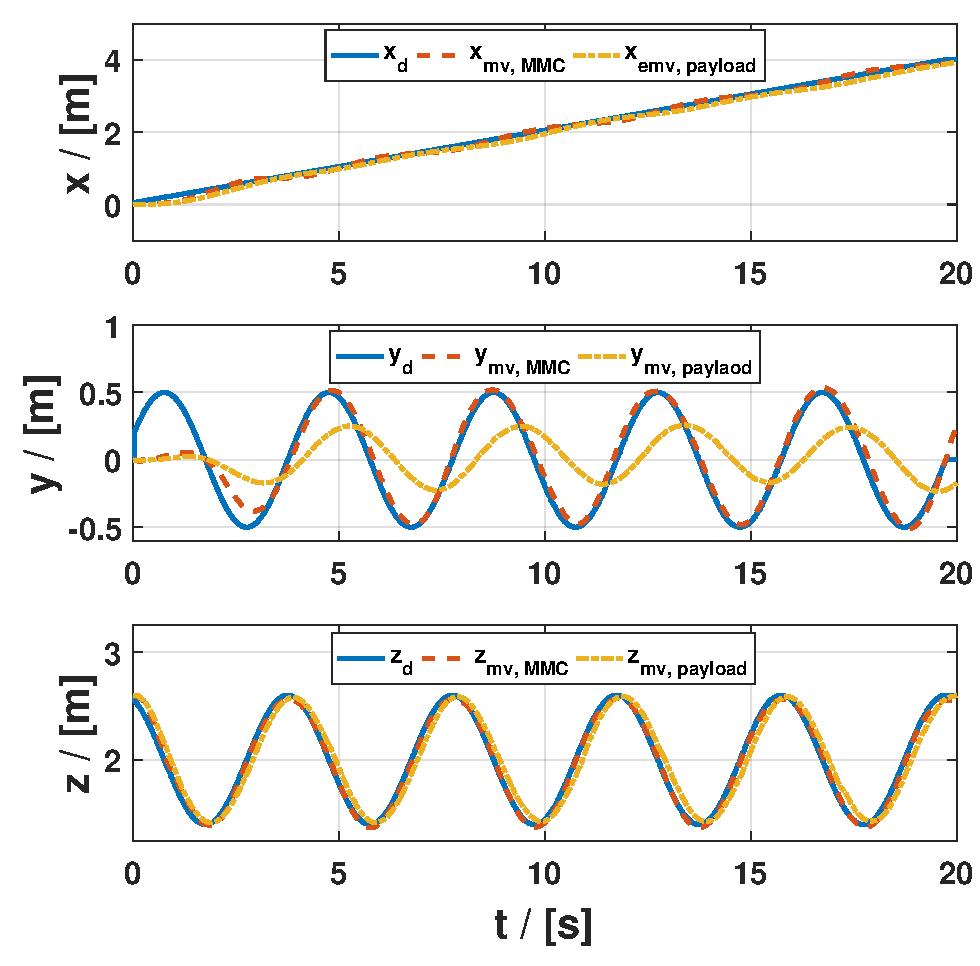
\includegraphics[width=0.8\columnwidth]{./pictures/both_pos_crop.pdf}
	\caption{Comparison between desired $\textbf{x}_d$ and measured position values $\textbf{x}_{mv}$ for both simulation cases. While tracking on x and z axes are reasonably similar, slower position tracking can be observed on the y axis for the second simulation case. Calculated MSE values are 0.0079 and 0.0352 for first and second case respectively.}
	\label{fig:traj_pos}
\end{figure}

\begin{figure}
	\centering
	\begin{minipage}{0.5\columnwidth}
		\centering
		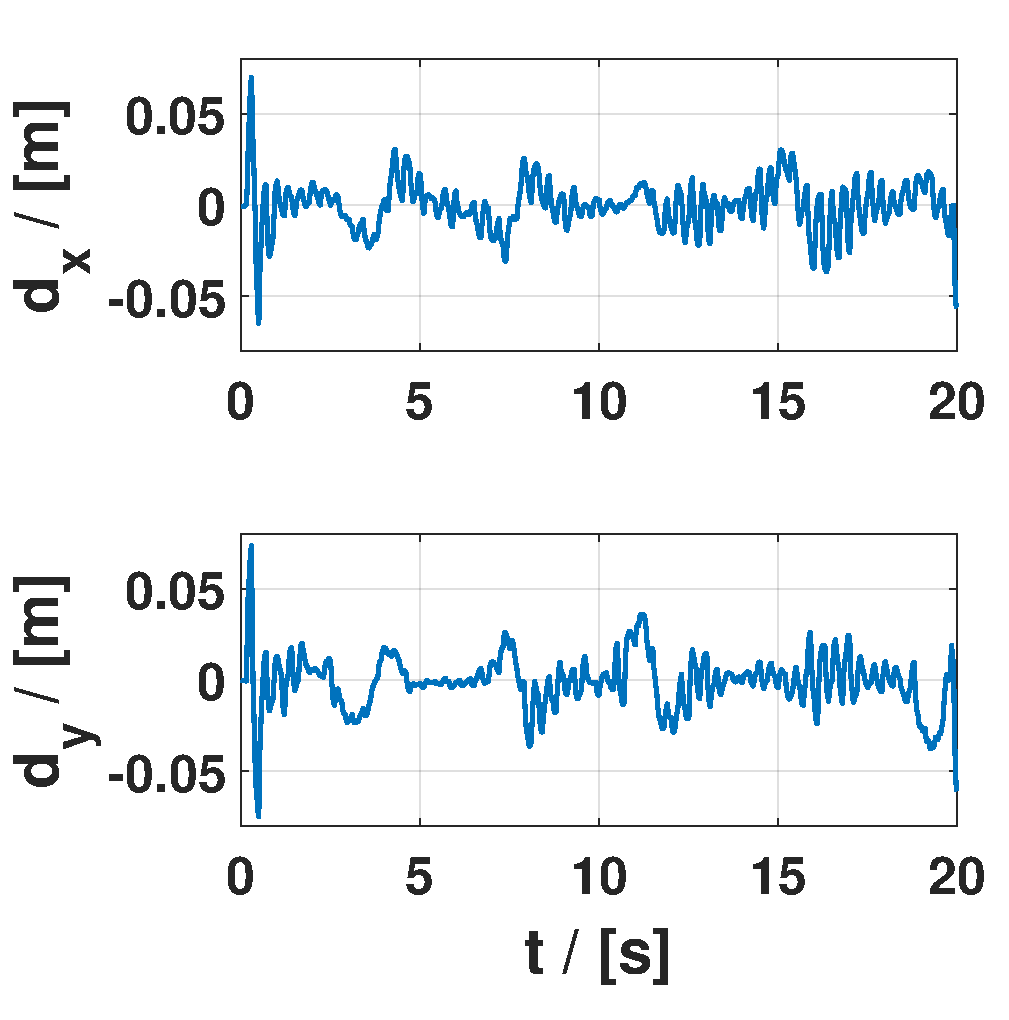
\includegraphics[width=\columnwidth]{./pictures/mmcuav_control_inputs_crop.pdf}
		\caption*{a) UAV with MMC}
		\label{fig:mmcuav_control}
	\end{minipage}%
	\begin{minipage}{0.5\columnwidth}
		\centering
		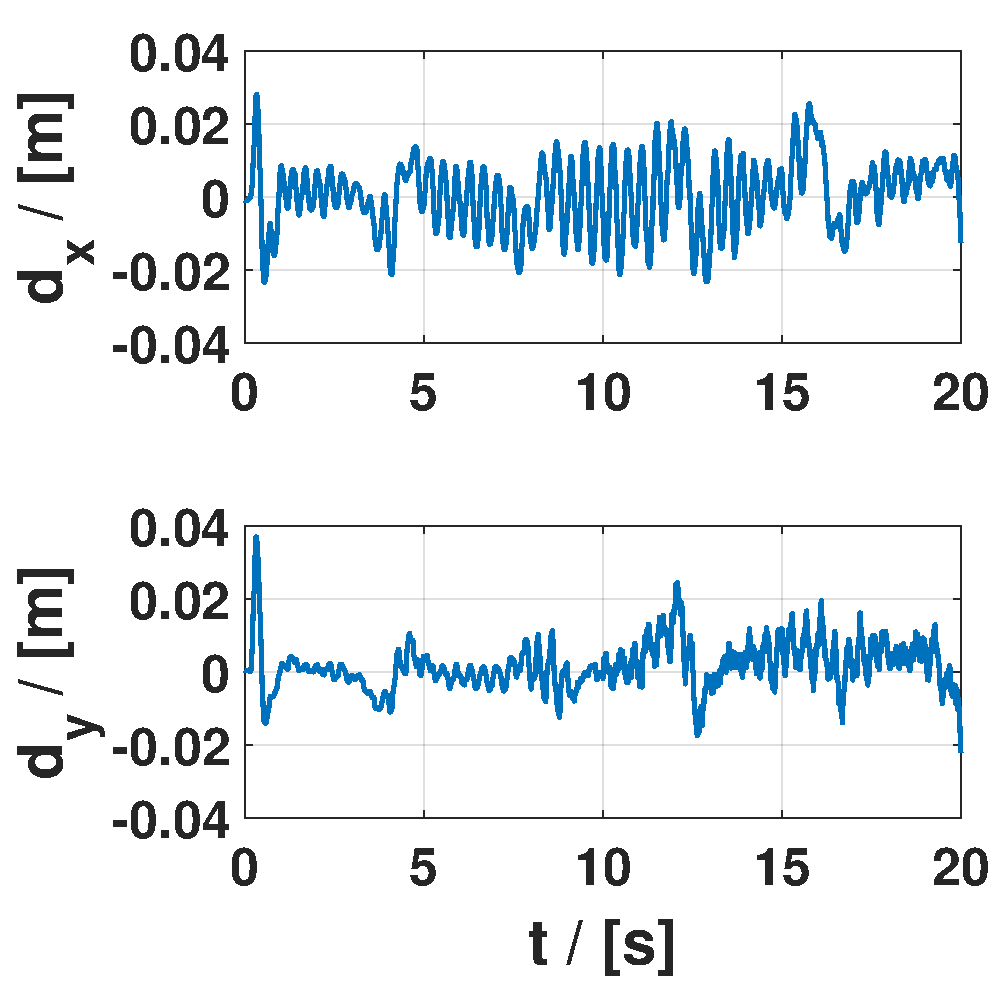
\includegraphics[width=\columnwidth]{./pictures/mmuav_control_inputs_crop.pdf}
		\caption*{b) UAV carrying a payload}
		\label{fig:mmuav_control}
	\end{minipage}
	\caption{Plot a) shows moving mass offsets w.r.t. the center of the UAV arms while plot b) shows payload movement in the body fixed frame. }
\end{figure}


\begin{figure}[h!]
	\centering
	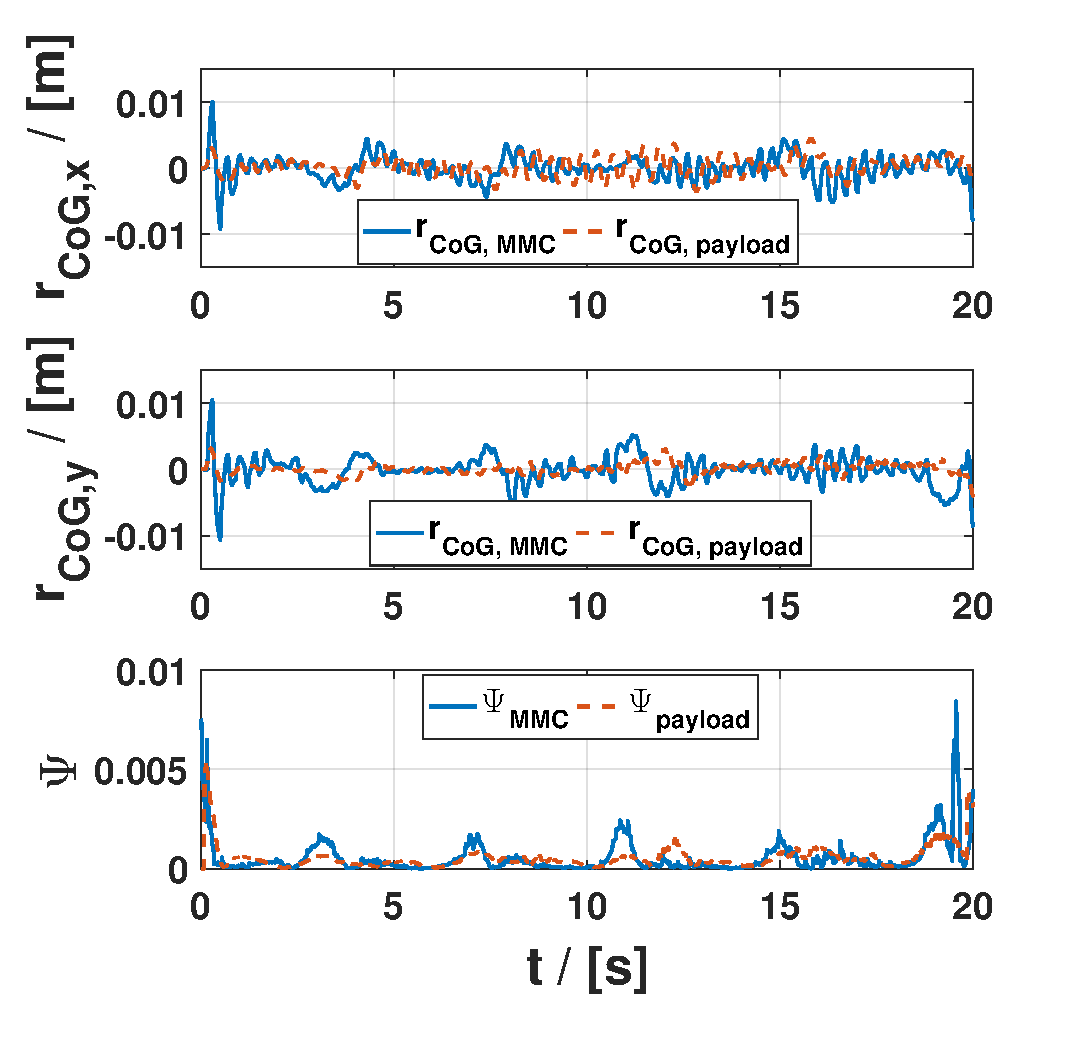
\includegraphics[width=0.9\columnwidth]{./pictures/cog_psi_crop.pdf}
	\caption{Comparison between first two components of CoG vector $\textbf{r}_{CoG}$ and between attitude error functions $\Psi$ for both simulation cases. It can be seen that higher magnitude of CoG variation can be achieved using moving masses rather than the carried payload.}
	\label{fig:cog_error}
\end{figure}


%\section{Experiments}
To demonstrate the proposed MMC-VPC control algorithm in action, we present the results of several experiments conducted on a real physical platform $\mu$MORUS, shown in Fig. \ref{fig:FlyingSCARA}. Our aerial robot is a 3D Robotics quadrotor equipped with four moving masses (NEMA 14 stepper motors) with a rack and pinion mechanism that transform rotational motion into linear motion. Masses are placed on each arm of the $\mu$MORUS platform. At the same time rotors are symmetrically placed around the central body in a pattern known as plus (+) configuration. We use a custom designed printed circuit board to command stepper motors and Pixhawk PX4 as the flight controller. For out first experiment we wanted to compare MMC-VPC control algorithm and classical rotor speed control in stabilization flight. We implemented MMC-VPC for pitch angle control while classical algorithm was controlling the roll angle. The second experiment was conducted to test the controller performance on simple trajectory. For that case, the MMC-VPC algorithm is implemented for both axis together with position controller. All control algorithms are implemented on the Pixhawk PX4 flight controller and the off-board computer is used for data logging. For testing purposes $\mu$MORUS is powered over electric cables and connected to the off-board computer through a USB cable.


%\subsection{Constrained 2DOF motion}

%First experiment was to test and tune control algorithm until satisfactory flight performance was achieved. To do so, we constrained $\mu$MORUS by mounting it on 2DOF gimbal. The sequence of commanded references and the response of vehicle’s pitch angle is presented in Fig. \ref{fig:pitch_kut_klackalica}. The MMC-VPC algorithm output is given in Fig. \ref{fig:polozaj_masa_klackalica}. Measured attitude data shows satisfying command tracking performance with RMS error of $0.038rad$, average overshoot of $27.5\%$ and average rise time $t_{r} = 0.32s$. The noise in moving masses motion is caused by rotor vibrations and unmodeled dynamics. Since we have shown that the moving masses are operating in higher bandwidth, they are responsible for initial, transient response, which one can observe in Fig. \ref{fig:pitch_kut_klackalica}. After certain amount of time, the MMC-VPC controller adjusts rotors' speed and the masses return to the center point of their operating range. This is identical to the results shown and discussed in Section \ref{sec:simulation}, and derived in Section \ref{sec:control}.

%\begin{figure}[h!]
%  \centering
%  \subfloat[]{\includegraphics[width=0.48\textwidth]{./pictures/%pitch_kut_klackalica}\label{fig:pitch_kut_klackalica}}
%  \hfill
%  \subfloat[]{\includegraphics[width=0.48\textwidth]{./pictures/polozaj_masa_klackalica}\label{fig:polozaj_masa_klackalica}}
%  \caption{Experimental results of $\mu$MORUS UAS on gimbal. a) shows a sequence of pitch references and the corresponding responses. b) shows a position setpoint of the moving masses and MMC-VPC control algorithm output for rotors.}
%\end{figure}

\subsection{Manual stabilization flight}

Our first experiment was manual stabilization flight with $\mu$MORUS. Pilot took-off with the vehicle, hovered for few minutes and then landed. Fig. \ref{fig:roll_pitch_kut_let} represents pitch and roll measurements during experiment. Considering attitude measurements in Fig. \ref{fig:roll_pitch_kut_let}, the results show that there is no significant difference between the two control paradigms. Results shows a stable flight, where both roll and pitch angles are within a few degrees. One has to be aware that the pilot was manually trying to keep the vehicle steady during the whole experiment, and that our goal was to show the proposed concept can stabilize the UAS in flight. The reference for MMC-VPC algorithm outputs, rotors 3 and 4, are given in Fig. \ref{fig:rc_out_let} alongside rotor 1 and rotor 2 which are controlled using the standard attitude controller. One can notice that the rotors commanded with MMC-VPC operate in lower bandwith. This is in line with the expected results, since the moving masses control attitude during the transient period which requires faster motion. This results with smother rotors' references, when compared to rotors 1 and 2. Nevertheless, the response of the UAV remains the same, as shown in Fig. \ref{fig:roll_pitch_kut_let}. The parameter used for attitude control loop are given in Table \ref{table:attitude_control_params}.

\begin{table}[h!]
\centering
\caption{MMC-VPC controller gains for attitude control loop where.}
\label{table:attitude_control_params}
\begin{tabular}{|c|c|c|c|c|c|c|}
\hline
 & $\phi$ & $\dot{\phi}$ & $\theta$ & $\dot{\theta}$ & $\psi$ & $\dot{\psi}$\\
\hline
$KP$ & $0$ & $0$ & $0$ & $0$ & $0$ & $0$\\
\hline
$KI$ & $0$ & $0$ & $0$ & $0$ & $0$ & $0$\\
\hline
$KD$ & $0$ & $0$ & $0$ & $0$ & $0$ & $0$\\
\hline
$KI_{VPC}$ & $0$ & $0$ & $0$ & $0$ & $0$ & $0$\\
\hline
\end{tabular}
\end{table}

\begin{figure}
  \centering
  \subfloat[]{\includegraphics[width=0.5\textwidth]{./pictures/pitch_kut_let}\label{fig:roll_pitch_kut_let}}
  \hfill
  \subfloat[]{\includegraphics[width=0.5\textwidth]{./pictures/rc_out_motor_ref_let}\label{fig:rc_out_let}}
  \caption{Experimental results of $\mu$MORUS UAS in stabilization flight. Roll and pitch measurements are depicted in a). b) shows reference for rotors 1-4. MMC-VPC takes higher bandwidth out of rotor 3 and 4 control, which results with smoother rotors' reference when compared to classically controlled rotors 1 and 2.}
\end{figure}

\subsection{Trajectory following}

The second experiment was conduced in order to test MMC-VPC algorithm with higher level control. We implemented position control in the standard cascade control form with PID controller. To tune our position controller we started with parameters from simulation and with some fine tuning we reached parameters shown in Table \ref{table:position_control_params}. 

\begin{table}[h!]
\centering
\caption{PID controller gains for cascade position control where $x$, $y$ and $z$ denotes outer control loop (position) and $vx$, $vy$ and $vz$ denotes inner control loop (velocity).}
\label{table:position_control_params}
\begin{tabular}{|c|c|c|c|c|c|c|}
\hline
 & $x$ & $vx$ & $y$ & $vy$ & $z$ & $vz$\\
\hline
$KP$ & $0$ & $0$ & $0$ & $0$ & $0$ & $0$\\
\hline
$KI$ & $0$ & $0$ & $0$ & $0$ & $0$ & $0$\\
\hline
$KD$ & $0$ & $0$ & $0$ & $0$ & $0$ & $0$\\
\hline
\end{tabular}
\end{table}

We can divide second experiment in to a two parts. The part a) of the experiment was to hover (maintain the constant position) with the $\mu$MORUS UAS and the part b) was to follow trajectory. On Fig. \ref{fig:position_hover} is shown position setpoint and feedback of the UAS while hovering. The UAS was able to maintain constant position with RMS error for position in x-axis $RMS_X = 0.0739 m$ and y-axis $RMS_Y = 0.0424 m$. The low level controller states for roll axis are shown on Fig. \ref{fig:roll_hover}, while pitch axis is almost identical. Here we can point out RMS error for roll angle $RMS_\phi = 2.091^{\circ}$ and RMS error for pitch angle $RMS_\theta = 2.354^{\circ}$.

\begin{figure}[h!]
\centering
\includegraphics[width=\columnwidth]{./pictures/arducopter_y_hover}
\caption{Results of the hovering experiment. Figure shows position setpoint and measurement for y-axis. Similar results are obtained for x-axis.}
\label{fig:position_hover}
\end{figure} 

\begin{figure}[h!]
  \centering
  \subfloat[]{\includegraphics[width=0.5\textwidth]{./pictures/arducopter_roll_hover}\label{fig:roll_hover}}
  \hfill
  \subfloat[]{\includegraphics[width=0.5\textwidth]{./pictures/arducopter_roll_rate_hover}\label{fig:rollrate_hover}}
  \caption{The experimental results of the $\mu$MORUS UAS during hovering experiment. a) shows a setpoints and the corresponding measurements for angle $\phi$. b) shows a setpoints and the corresponding measurements for angular velocity $\dot{\phi}$. The results for $\theta$ angle are similar.}
  \label{fig:roll_hover}
\end{figure}

The b) part of the experiment (following a trajectory) give us a position results that are shown on Fig. \ref{fig:experiment_position}. The UAS was able to follow trajectory with RMS error $RMS = 0.3139 m$. The roll angle and roll rate during the trajectory execution are shown on Fig. \ref{fig:experiment_roll}. The video showing both experiments can be found in \cite{uMORUS2017video}. The Github repository with source code for both simulation can bi found in \cite{letaci2017} and experiments in \cite{letaciPixhawk2017}.

\begin{figure}[h!]
\centering
\includegraphics[width=\columnwidth]{./pictures/arducopter_y}
\caption{Results of the trajectory following. Figure shows position setpoint and measurement for y-axis. Similar results are obtained for x-axis.}
\label{fig:experiment_position}
\end{figure}


\begin{figure}[h!]
  \centering
  \subfloat[]{\includegraphics[width=0.5\textwidth]{./pictures/arducopter_roll}\label{fig:experiment_roll_angle}}
  \hfill
  \subfloat[]{\includegraphics[width=0.5\textwidth]{./pictures/arducopter_roll_rate}\label{fig:experiment_roll_rate}}
  \caption{The experimental results of the $\mu$MORUS UAS during the trajectory following experiment. a) shows a setpoints and the corresponding measurements for angle $\phi$. b) shows a setpoints and the corresponding measurements for angular velocity $\dot{\phi}$. The results for $\theta$ angle are similar.}
  \label{fig:experiment_roll}
\end{figure}
\section{Conclusion}

\todo[inline]{Conclusions}



%%%%%%%%%%%%%%%%%%%%%%%%%%%%%%%%%%%%%%%%%%%%%%%%%%%%%%%%%%%%%%%%%%%%%%%%%%%%%%%%
\section*{APPENDIX}
In this section rotating body dynamics with variations in center of gravity is derived.
General form of Euler-Lagrange dynamics for a rotating rigid body on SE(3) configuration manifold in the body-fixed frame as presented in \cite{LeeModel}:

\begin{gather}
	\frac{d}{dt} \left( \frac{\partial \La}{\partial \mb{\Omega}} \right)
	+ \mb{\Omega} \times \frac{\partial \La}{\partial \mb{\Omega}} 
	+ \textbf{v} \times \frac{\partial \La}{\partial \textbf{v}} 
	+ \sum_{i=1}^{3} \textbf{r}_i \times \frac{\partial \La}{\partial \textbf{r}_i} = 0 \label{general1}\\
	\frac{d}{dt} \left( \frac{\partial \La}{\partial \textbf{v}} \right)
	+ \mb{\Omega} \times \frac{\partial \La}{\partial \textbf{v}} 
	- \text{R}^T \frac{\partial \La}{\partial x} = 0 \label{general2}
\end{gather}
For the proposed UAV with variations in CoG the Lagrangian is:

\begin{gather}
\begin{align}
\begin{split}
	\La(\text{R},x,\mb{\Omega},\textbf{v}) &= \frac{1}{2}\mb{\Omega}^T\text{J}\mb{\Omega} \,+\, m \mb{\Omega}^T \reallywidehat{\textbf{r}}_{CoG}\textbf{v} \\
	\, &+\, \frac{1}{2}m\textbf{v}^T\textbf{v} \,-\, U(\text{R},\textbf{x}) \, ,
\end{split}
\end{align}
\end{gather}
where $U(\text{R}, \textbf{x})$ is the potential energy. It is important to note that \text{J} and $\textbf{r}_{CoG}$ are variable over time. \\
%Lagrangian derivatives needed for the general form equations \ref{general1} and \ref{general2} are:
%\begin{gather}
%	\frac{\partial \La}{\partial \mb{\Omega}} = \text{J}\mb{\Omega} + m \reallywidehat{\textbf{r}}_{CoG}\textbf{v} \label{d1}\\ 
%	\frac{d}{dt} \left( \frac{\partial \La}{\partial \mb{\Omega}} \right) = \dot{\text{J}} \mb{\Omega} + \text{J} \dot{\mb{\Omega}} + m \dot{\textbf{r}}_{CoG} \times \textbf{v} + m \textbf{r}_{CoG} \times \dot{\textbf{v}} \label{d2}\\ 
%	\frac{\partial \La}{\partial \textbf{v}} = m\textbf{v} - m\textbf{r}_{CoG} \times \mb{\Omega} \label{d3}\\ 
%	\frac{d}{dt} \left( \frac{\partial \La}{\partial \textbf{v}} \right) = m\dot{\textbf{v}} - m\dot{\textbf{r}}_{CoG} \times \mb{\Omega} - m \textbf{r}_{CoG} \times \dot{\mb{\Omega}} \label{d4}
%\end{gather}
It is of interest to transfer rotation and translation dynamics in the inertial frame. This can be done using the following relations:
\begin{gather}
	\textbf{v} = \text{R}^T \dot{x} \label{inertial1}\\
	\dot{\textbf{v}} = \text{R}^T \ddot{\textbf{x}} - \mb{\Omega} \times (\, \text{R}^T \dot{\textbf{x}} \,) \label{inertial2} \\
	\textbf{r}_{CoG} = \text{R}^T(\, \textbf{x}_{CoG} - \textbf{x} \,) \label{inertial3} \\
	\dot{\textbf{r}}_{CoG} = \text{R}^T(\, \dot{\textbf{x}}_{CoG} - \dot{\textbf{x}} \,) - \reallywidehat{\mb{\Omega}}\text{R}^T(\, \textbf{x}_{CoG} - \textbf{x} \,) \label{inertial4}
\end{gather}
After computing Lagrangian derivatives, plugging them in \ref{general1}, \ref{general2} and using \ref{inertial1}, \ref{inertial2} as velocity and acceleration transformations to the inertial frame the following equations are obtained:
\begin{gather}
\label{complete_model1}
\begin{align}
	\begin{split}
		\text{J}\dot{\mb{\Omega}} &+ m \textbf{r}_{CoG} \times \text{R}^T \ddot{\textbf{x}} + \mb{\Omega} \times \text{J}\mb{\Omega} \\
		&+ \dot{\text{J}} \mb{\Omega} + m \dot{\textbf{r}}_{CoG} \times \text{R}^T \dot{\textbf{x}} + \sum_{i=1}^{3} \textbf{r}_i \times \frac{\partial \La}{\partial \textbf{r}_i} = 0
	\end{split}
\end{align}
\end{gather}
\begin{gather}
\label{complete_model2}
\begin{align}
	\begin{split}
		m \ddot{\textbf{x}} & - m \text{R} \,(\, \textbf{r}_{CoG} \times \dot{\mb{\Omega}} \,) - m \text{R} \,[\, \mb{\Omega} \times (\, \textbf{r}_{CoG} \times \mb{\Omega} \,) \,] \\
		&- m \text{R} \,(\, \dot{\textbf{r}}_{CoG} \times \mb{\Omega} \,) + \frac{\partial U(\text{R},\textbf{x})}{\partial \textbf{x}} = 0
	\end{split}
\end{align}
\end{gather}
Finally, CoG transforms \ref{inertial3} and \ref{inertial4} are included along with forces and moments acting in the body-fixed frame which gives the following model dynamics:
\begin{gather}
\begin{align}
	\begin{split}
		 \text{J}\dot{\mb{\Omega}} & + m \textbf{r}_{CoG} \times \text{R}^T\ddot{\textbf{x}} + \mb{\Omega} \times \text{J}\mb{\Omega}  \\
		 & - m (\, \mb{\Omega} \times \textbf{r}_{CoG} \,) \times \text{R}^T \dot{\textbf{x}} \\
		 & + \dot{\text{J}}\mb{\Omega} + m \, \reallywidehat{R^T (\, \dot{\textbf{x}}_{CoG} - \dot{\textbf{x}} \,)} \, R^T\dot{\textbf{x}} = \textbf{M}
	\end{split}
\end{align}
\end{gather}
\begin{gather}
\begin{align}
	\begin{split}
		m \ddot{\textbf{x}} & - m \text{R} \,(\, \textbf{r}_{CoG} \times \dot{\mb{\Omega}} \,) + m g\textbf{e}_3 \\
		& - m \text{R} \, \reallywidehat{ \text{R}^T (\, \dot{\textbf{x}}_{CoG} - \dot{\textbf{x}} \,) } \, \mb{\Omega}  = f\text{R}\textbf{e}_3
	\end{split}
\end{align}
\end{gather}
\noindent Please note that \textit{wide hat} is the same operator previously defined in \eqref{eqn:hat}.

%Appendixes should appear before the acknowledgment.

\section*{ACKNOWLEDGMENT}

This research was supported in part by NATO's Emerging Security Challenges Division in the framework of the Science for Peace and Security Programme as Multi Year Project under G. A. number 984807, named Unmanned system for maritime security and environmental monitoring - MORUS.


%%%%%%%%%%%%%%%%%%%%%%%%%%%%%%%%%%%%%%%%%%%%%%%%%%%%%%%%%%%%%%%%%%%%%%%%%%%%%%%%

\nocite{*}
\bibliographystyle{ieeetr}
\bibliography{bibliography/Mendeley}

\end{document}
